%%% LaTeX Template: Two column article
%%%
%%% Source: http://www.howtotex.com/
%%% Feel free to distribute this template, but please keep to referal to http://www.howtotex.com/ here.
%%% Date: February 2011

%%% Preamble
\documentclass[	DIV=calc,%
							paper=a4,%
							fontsize=11pt,%
							twocolumn]{scrartcl}	 					% KOMA-article class

\usepackage{lipsum}	
% Package to create dummy text

\usepackage[english]{babel}										% English language/hyphenation
\usepackage[protrusion=true,expansion=true]{microtype}				% Better typography
\usepackage{amsmath,amsfonts,amsthm}					% Math packages
\usepackage[pdftex]{graphicx}									% Enable pdflatex
\usepackage[svgnames]{xcolor}									% Enabling colors by their 'svgnames'
\usepackage[hang, small,labelfont=bf,up,textfont=it,up]{caption}	% Custom captions under/above floats
\usepackage{epstopdf}												% Converts .eps to .pdf
\usepackage{subfig}													% Subfigures
\usepackage{booktabs}												% Nicer tables
\usepackage{fix-cm}	
\definecolor{AirForceBlue}{rgb}{0.36, 0.54, 0.66}
% Custom fontsizes



%%% Custom sectioning (sectsty package)
\usepackage{sectsty}													% Custom sectioning (see below)
\allsectionsfont{%															% Change font of al section commands
	\usefont{OT1}{phv}{b}{n}%										% bch-b-n: CharterBT-Bold font
	}

\sectionfont{%																% Change font of \section command
	\usefont{OT1}{phv}{b}{n}%										% bch-b-n: CharterBT-Bold font
	}



%%% Headers and footers
\usepackage{tcolorbox}
\usepackage{fancyhdr}	
% Needed to define custom headers/footers
	\pagestyle{fancy}														% Enabling the custom headers/footers
\usepackage{lastpage}	

% Header (empty)
\lhead{}
\chead{}
\rhead{}
% Footer (you may change this to your own needs)
\lfoot{\footnotesize \texttt{1st Order Kinetics: Worked Examples} \textbullet ~C. Batchelor-McAuley}
\cfoot{}
\rfoot{\footnotesize page \thepage\ of \pageref{LastPage}}	% "Page 1 of 2"
\renewcommand{\headrulewidth}{0.0pt}
\renewcommand{\footrulewidth}{0.4pt}



%%% Creating an initial of the very first character of the content
\usepackage{lettrine}
\newcommand{\initial}[1]{%
     \lettrine[lines=3,lhang=0.3,nindent=0em]{
     				\color{AirForceBlue}
     				{\textsf{#1}}}{}}

%%% Title, author and date metadata
\usepackage{titling}															% For custom titles

\newcommand{\HorRule}{\color{Black}%			% Creating a horizontal rule
									  	\rule{\linewidth}{1pt}%
										}


\pretitle{\vspace{-50pt} \begin{flushleft} \HorRule 
				\vspace{10pt}\fontsize{30}{30} \usefont{OT1}{phv}{b}{n} \color{AirForceBlue} \selectfont }
				

\title{1st Order Kinetics:\\Worked Examples}					% Title of your article goes here
\posttitle{\par\end{flushleft}\vskip 0.5em}

\preauthor{\begin{flushright}
\vspace{-40pt}
					\large \lineskip 0.5em \usefont{OT1}{phv}{b}{sl} \color{AirForceBlue}}											% Author name goes here
\postauthor{\footnotesize \usefont{OT1}{phv}{m}{sl} \color{Black} 
								% Institution of author
					\par\end{flushright}\HorRule}

\date{}																				% No date
\setlength{\textfloatsep}{0.1\textfloatsep}
%%% Begin document
\begin{document}
\twocolumn[
   \begin{@twocolumnfalse} 
     \maketitle
          \vspace{-40pt}

    \begin{tcolorbox}
        \begin{itemize}
             \setlength\itemsep{0.2em}
             \item{Radioactive decay follows first order kinetics and can be used to find the age of a material}
             
             \item{Most chemical reactions do not follow first order kinetics but can, in some cases, be made to follow pseudo-first order kinetics}
        
        \end{itemize}  
    \end{tcolorbox}
\shiftup
     \vspace{-10pt}
     
     ~\newline
    \end{@twocolumnfalse}
]
\thispagestyle{fancy} 			% Enabling the custom headers/footers for the first page 
% The first character should be within \initial{}
\setlength{\abovedisplayskip}{6pt}
\setlength{\belowdisplayskip}{6pt}

\subsection*{Example 1\\Radioactive Decay: $^{14}$C}
\begin{quote}
    \normalsize{``... the investigation of human history through the use of chemistry ..."}
    \\\emph{W.~Libby}
\end{quote}
Carbon has two stable isotopes: $^{12}\mathrm{C}$ and $^{13}\mathrm{C}$. 98.9\% of terrestrial carbon is $^{12}\mathrm{C}$, 1.1\% is $^{13}\mathrm{C}$ and there are trace levels of $^{14}\mathrm{C}$. $^{14}\mathrm{C}$ is formed indirectly by high energy cosmic rays entering the atmosphere. Once formed, the $^{14}\mathrm{C}$ goes through beta decay to $^{14}\mathrm{N}$ with the emission of an electron and an antineutrino. The half-life of this decay process is 5730$\pm$40 yr. Although only present at trace levels the relative abundance (concentration) of $^{14}\mathrm{C}$ in the atmosphere is reasonably constant; the rate of loss of $^{14}\mathrm{C}$ by beta decay is virtually fully compensated for by the formation of new $^{14}\mathrm{C}$ such that we are in a steady state situation. When a plant or animal is alive it constantly exchanges carbon with the atmosphere; plants convert CO$_2$ to sugars, animals eat the plants and release CO$_2$ via respiration. While something is living, then, it contains the same amount of $^{14}\mathrm{C}$ as is found in the atmosphere. But once it dies, it no longer exchanges carbon with the atmosphere; consequently, the quantity of $^{14}\mathrm{C}$ it contains decreases as a function of time. Therefore by either directly or indirectly measuring the concentration of  $^{14}\mathrm{C}$ in a sample it is possible to determine when it died.

Classically, carbon dating was undertaken by using a highly sensitive Geiger counter (Fig \ref{fig:device}) to measure the $^{14}\mathrm{C}$ decay rate. Modern measurements are achieved using an accelerator mass spectrometer.

~
\newline
\textbf{Q.} What are the advantages of using \newline mass spectrometry for carbon dating?

\newpage
Using a device similar to that presented in Fig \ref{fig:device} it was discovered that carbon sourced from living (or recently living) material decays at an average rate of 13.56$\pm$0.07 decays per minute per gram of carbon (atoms min$^{-1}$ gC$^{-1}$). 

~
\newline
\textbf{From this decay rate and the half-life of the material how can we determine the long-term ratio of $^{14}\mathrm{C}$ to $^{12}\mathrm{C}$ in the atmosphere?}

\begin{figure}
    \centering
    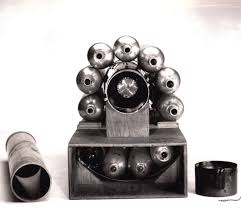
\includegraphics{libby.jpeg}
    \captionsetup{format=plain}
    \caption{An early $^{14}$C dating device produced by W.Libby, owned by the Smithsonian Institute. The central cylinder contains a sensitive Geiger counter, surrounded by co-incident Geiger counters, used to rule out false positives due to cosmic rays.}
    \label{fig:device}
\end{figure}
\\
\\
To answer this question we need to recognise a few things. First, although it's not in units we're used to, the rate of decay we've been given has the dimension of quantity per time; it's telling us how many atoms of $^{14}\mathrm{C}$ per gram of carbon are being converted to $^{14}\mathrm{N}$ in a minute. We can express the rate as:
\begin{equation}
    \nu = -\frac{dN}{dt}
\end{equation}
where here N is the number of atoms per gram of carbon (atoms gC$^{-1}$). Second, the carbons decay independently, and consequently the rate of decay follows first order kinetics:
\begin{equation}
    \nu = kN 
\end{equation}
k is the decay rate constant (time$^{-1}$).
Third, we've been given a half-life in years, we need to convert this to a rate constant and convert the units to min$^{-1}$.

\begin{align}
    k &= \frac{\ln(2)}{t_{1/2}} \\
     &= \frac{\ln2}{5730*365.24*24*60} \\
     &= 2.3\times10^{-10}~\mathrm{min}^{-1}
\end{align}
Taking the expression for the first order rate law we have:
\begin{equation}
    \frac{dN}{dt} = -kN
    \label{eq:c14d}
\end{equation}
If we note that only a \emph{very} small fraction of the carbon atoms decay during the course of the measurement then we can treat the number as a constant (this is a bit of a cheat; see the information box on initial rates for more details). Substituting our above values into equation \ref{eq:c14d} gives:
\begin{align}
    13.56 &= 2.3\times10^{-10} N\\
    N &= 5.9\times 10^{10} \mathrm{atoms~gC^{-1}}
\end{align}
The only task left is to calculate the number of atoms of carbon in one gram.
Hence:
\begin{equation}
    ^{14}\mathrm{C}:{^{12}\mathrm{C}} = 1.2\times10^{-12}
\end{equation}

~
\newline
\textbf{Q.} A sample of carbon was determined to have a $^{14}$C decay rate of 1.7 atoms min gC$^{-1}$. How old was the sample?


\subsection*{Example 2\\Hydrogen Peroxide disproportionation}
Although thermodynamically favorable, in the absence of a catalyst the decomposition of $\mathrm{H_2O_2}$ is very slow. A bottle of 30\% $\mathrm{H_2O_2}$ can remain in the fridge for months. $\mathrm{H_2O_2}$ absorbs strongly in the UV part of the electromagnetic spectrum hence by monitoring the absorbance of light at 240 nm the peroxide concentration in a solution can be measured. 

Platinum is an excellent catalyst for the decomposition of hydrogen peroxide. Figure \ref{fig:TEM} depicts a representative transmission electron microscope image for a sample of mesoporous 50 nm nanoparticles. 
%\begin{figure}
    \begin{tcolorbox}[colback=blue!5,colframe=AirForceBlue!100!black,title=Initial Rates]
      If the concentration of a reactant only changes a very small amount over the course of a measurement, rather than integrating the associated rate law one may treat the unknown (the concentration of the reactant) as a constant. This `trick' is often used when measuring the so-called initial reaction rate but, for a first order reaction, can we justify this approach a \emph{little} more rigorously? 
      
      As an alternative what happens if we don't assume the concentration of the reactant to be a constant but assume that it varies linearly as a function of time, i.e. we  are assuming that the rate of the reaction is constant.
      If the initial concentration of a reactant is $c_{A,0}$ then after time t this concentration will have decreased to approximately ($c_{A,0} - \nu t$) if we substitute these two concentrations into the first order integrated rate law we get:
      \begin{equation}
          \frac{c_{A,0} - \nu t}{c_{A,0}} = e^{-kt}
      \end{equation}
      For small values of x:
      \begin{equation}
          e^{x} \approx 1 + x
          \label{eq:powerseries}
      \end{equation}
      Eq. \ref{eq:powerseries} comes from expressing the exponential as a power series where we ignore anything greater than the linear ($x^1$) term. Hence,
      \begin{align}
          1-\frac{\nu t}{c_{A,0}} &= 1 - k t \\
          \frac{\nu}{k} &= c_{A,0}
      \end{align}
      The above approximation is exactly the one we use in Example 1 to determine the quantity of $^{14}$C in the atmosphere.
    \end{tcolorbox}
%\end{figure}

\begin{figure}
    \centering
    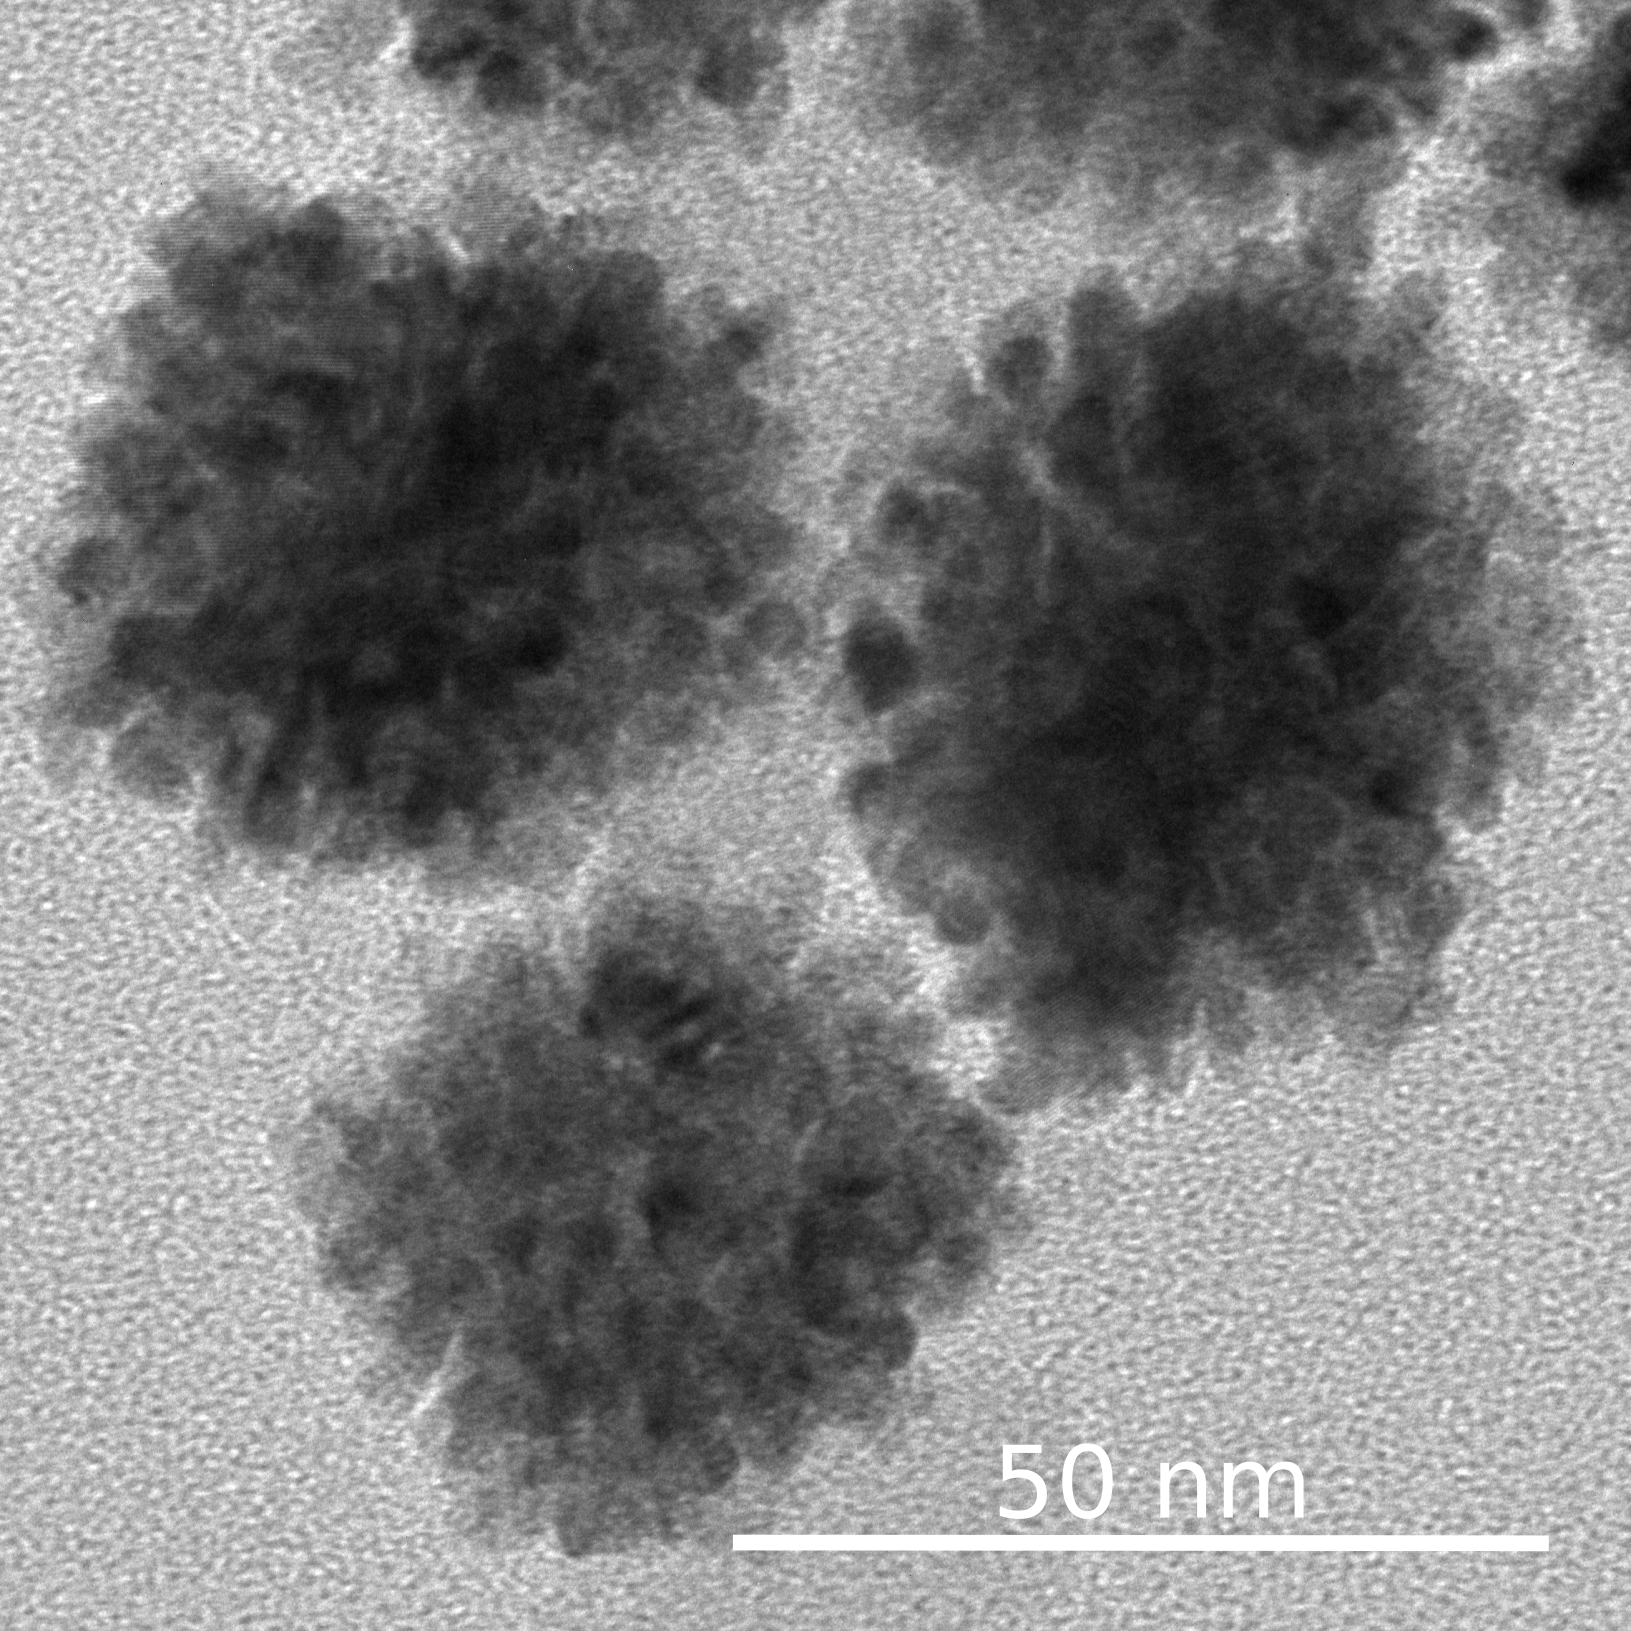
\includegraphics[width=\linewidth]{TEM_kin.png}
    \captionsetup{format=plain}
    \caption{Transmission electron microscope image of a sample of 50 nm mesoporous platinum nanoparticles. The image shows that the particles are formed from the aggregation of small \~ 5 nm crystallites.}
    \label{fig:TEM}
\end{figure}

\noindent A solution initially containing 1.25 mM hydrogen peroxide and a variable concentrations of platinum nanoparticles was made up and the change in the peroxide concentration monitored as a function of time.  
Table \ref{H2O2vals} gives the measured concentration of hydrogen peroxide at three different times after mixing of the solution. The rate law for this process is:
\begin{equation}
    \nu = k c_{H_2O_2} c_{NP}
\end{equation}
where $C_{NP}$ is the solution phase nanoparticle concentration. 
Calculate the rate constant (k) for the reaction (the information box on pseudo first order kinetics may help).

\begin{table}[h]
    \begin{tabular}{l|lll}
        Time /s & \multicolumn{3}{l}{NP Concentration / pM} \\
         & 0.4 & 1.6 & 3.2 \\
         \hline
         50 & 1.22 & 1.15 & 1.05 \\
         100 & 1.20 & 1.05 & 0.88 \\
         150 & 1.17 & 0.96 & 0.74 \\
         200 & 1.15 & 0.87 & 0.62
    \end{tabular}
    \captionsetup{format=plain}
    \caption{Hydrogen peroxide concentration (mM) as measured as a function of time in a solution initially containing 1.25 mM hydrogen peroxide and variable concentrations of nanoparticles as } 
    \label{H2O2vals}
\end{table}
From the given rate law for the reaction and the stoichiometry of the reaction:
\begin{equation}
    \frac{d c_{H_2O_2}}{dt} = -2kc_{H_2O_2}c_{NP}
\end{equation}

\noindent as the nanoparticles are a catalyst their concentration is constant during the reaction. Hence integrating the above rate law we have:
\begin{equation}
    \ln{\frac{c_{H_2O_2,t}}{c_{H_2O_2,0}}} = -2kc_{NP}t
\end{equation}
Consequently, a plot of $\ln{\frac{c_{H_2O_2,t}}{c_{H_2O_2,0}}}$ versus time should yield a straight line with a gradient of $-2kc_{NP}$. The data presented in table 1 is plotted in Figure and from the gradients the rate constant for the platinum nanoparticle catalysed disproportionation of hydrogen peroxide is found to be $k = 5.4 \times 10^8$ mol$^{-1}$ dm$^{3}$ s$^{-1}$.
 a straight line with a gradient of $-2kc_{NP}$. The data presented in table 1 is plotted in Figure and from the gradients the rate constant for the platinum nanoparticle catalysed disproportionation of hydrogen peroxide is found to be $k = 5.4 \times 10^8$ mol$^{-1}$ dm$^{3}$ s$^{-1}$.
\begin{figure}
    \centering
    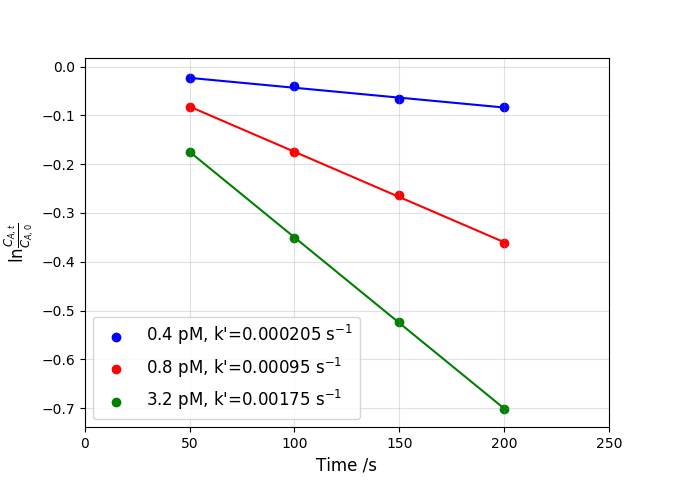
\includegraphics[width=\linewidth]{figure_2.png}
    \captionsetup{format=plain}
    \caption{1st Order reaction rate plot for the decomposition of hydrogen peroxide (c$_{{H_2O_2},0}$ = 1.25 mM) catalysed by platinum nanoparticles of concentration 0.4, 1.6 and 3.2 pM. k' is the measured pseudo-first order reaction rate in which the reaction stoichiometry has been accounted for.}
    \label{fig:rate}
\end{figure}

As can be seen from the transmission electron microscopy images the used nanoaprticles are not smooth solid structures. It is difficult to determine i) the nanoparticle surface area and ii) how chemically accessible internal porous surfaces may be. In many experimental situations the rate of the hydrogen peroxide decomposition reaction is found to be proportional to the platinum surface area. Consequently, this catalytic decomposition reaction was recently studied on this material as one method by which the porosity of the nanoparticles could be studied; the measured rate constant is related to the nanoparticle surface area. From this is was possible to evidence that for these particles the internal nanoparticle surface structure actively participates in the catalytic reaction.
~
\\

\begin{figure}[h]
    \begin{tcolorbox}[[colback=red!5,colframe=red!40!black, title=Looking Forward: Transition State Theory]
        The above discussion of first order kinetics feeds into a number of subjects not least photochemistry where it is important for understanding the rate of photo-luminescent processes. However, in terms of developing our understanding of kinetics one of the big subjects is moving beyond an empirical understanding of the effect of temperature on the rate of a reaction, as described by the Arrhenius equation, and towards a molecular view as provided by Transition State Theory (see Chapter 18C of \emph{Atkins Physical Chemistry, 11 Ed.})
    \end{tcolorbox}
\end{figure}


\newpage
    \begin{tcolorbox}[colback=blue!5,colframe=AirForceBlue!100!black,title= Pseudo-First Order]
        Most chemical processes don't generally follow first order reaction kinetics; however, it's sometimes possible to contrive the experimental conditions so that the reaction rate approximates to that of a first order reaction a.k.a. making the reaction pseudo-first order. This can be a helpful technique as it can simplify the reaction kinetics and make it easier to quantitatively analyse the chemical reaction.
        Take the second order rate law for the reaction between species A and B:
        \begin{equation}
            \nu = k c_A c_B
        \end{equation}
        if an excess of the reactant B is used then during the course of the reaction its concentration will not change significant hence we can take $C_B$ as a constant. In this case the rate law becomes pseudo first order:
        \begin{equation}
            \nu = k' c_A
        \end{equation}
        where $k'$ has units of s$^{-1}$ and is equal to $kc_B$. It is important to note that the measured pseudo-first order rate constant varies as a function of the concentration of B.
    \end{tcolorbox}

\end{document}